\documentclass{beamer}

%Rajouter les slides de photoélasticité à fin

%%%%%%%%%%%%%%%%%%%%%%%%%%%%%
% Tikz packages and settings
%%%%%%%%%%%%%%%%%%%%%%%%%%%%%

\usepackage{tikz}
\usepackage{pgfplots}
\usepackage{tikz-3dplot}
\pgfplotsset{compat=1.11}

\usetikzlibrary{shapes.geometric,calc,intersections}
\usetikzlibrary{shapes.arrows}
\usetikzlibrary{shadings}
\usetikzlibrary{patterns}
\usetikzlibrary{decorations.pathmorphing}
\usetikzlibrary{decorations.pathreplacing}


\usetikzlibrary{external}
\tikzset{external/aux in dpth={false}}
\tikzset{external/up to date check={simple}}
\tikzset{external/optimize command away={\includetexgraphics}{2}}

\tikzset{>=stealth}

%%%%%%%%%%%%%%%%%%%%%%%%%%%%%%%%%%%%%%%%%%%%%%%%%%%%%%%%%%%%
% Custom macro to input a tikz picture and setting its name
%%%%%%%%%%%%%%%%%%%%%%%%%%%%%%%%%%%%%%%%%%%%%%%%%%%%%%%%%%%%

\makeatletter
\newcommand{\includetikzgraphics}[1]{
	\filename@parse{#1}
	\tikzsetnextfilename{\filename@base}
	\input{#1}
}
\makeatother

%%%%%%%%%%%%%%%%%%%%%%%%%%%%%%%%%%
% Custom tikz command for drawing
%%%%%%%%%%%%%%%%%%%%%%%%%%%%%%%%%%

\tikzset{math3d/.style=
    {z= {(-0cm,-0.3cm)}, y={(0cm,1cm)},x={(1cm,0cm)}}}

% \drawYNema {x} {y} {yAngle}
\newcommand{\drawYnema}[3] {
	\shade [ball color=black] (#1,#2) ellipse 
		[x radius={sqrt(pow(cos(#3)*0.1,2)+pow(sin(#3)*0.3,2))}, y radius=0.1];
}
% \drawXNema {x} {y} {xAngle}
\newcommand{\drawXnema}[3] {
	\shade [ball color=black] (#1,#2) ellipse 
		[y radius={sqrt(pow(cos(#3)*0.1,2)+pow(sin(#3)*0.3,2))}, x radius=0.1];
}
% \drawZNema {x} {y} {zAngle}
\newcommand{\drawZnema}[3] {
	\shade [ball color=black] (#1,#2) ellipse 
		[x radius=0.3, y radius=0.1, rotate={#3}];
}

% \plotcylinder { radius } { heigth } { altitude }
\newcommand{\plotcylinder}[3] {
     \draw [math3d, fill=white, samples=100]
        plot[domain=-pi:pi] ({#1*cos(\x r)},#3,{#1*sin(\x r)}) ;
     \draw [math3d, fill=white, samples=100]
        plot[domain=0:pi] ({#1*cos(\x r)},#3,{#1*sin(\x r)}) --
        plot[domain=pi:0] ({#1*cos(\x r)},{#3-#2},{#1*sin(\x r)}) --
        cycle;
}

% \plotpolarizer { x} { y} { z } { radius } { angle }
\newcommand{\plotpolarizer}[5] {
    \draw [math3d, fill=gray, opacity=0.8, samples=100]
        plot[domain=-pi:pi] ({#1+#4*cos(\x r)},#2,{#3+#4*sin(\x r)}) ;
    \draw [math3d, opacity=0.8]
        ({#1+#4*cos(#5)},#2,{#3+#4*sin(#5)}) -- ({#1-#4*cos(#5)},#2,{#3-#4*sin(#5)}) ;
}

% \fancyarrow {xi} {yi} {xf} {yf} {width} {options}
\newcommand{\fancyarrow}[6]{
	\pgfmathsetmacro{\dx}{#3-#1};
	\pgfmathsetmacro{\dy}{#4-#2};
	\pgfmathsetmacro{\dl}{sqrt(\dx*\dx+\dy*\dy)};
	\pgfmathsetmacro{\dw}{#5/2};
	\pgfmathsetmacro{\cos}{\dx/\dl};
	\pgfmathsetmacro{\sin}{\dy/\dl};
	\draw [#6] (#1,#2) -- ++($\dw*(\sin,-\cos)$) 
		-- ++(${\dl-2*\dw}*(\cos,\sin)$)
		-- ++($\dw*(\sin,-\cos)$) -- ++($2*\dw*(\cos,\sin)+2*\dw*(-\sin,\cos)$) 
		-- ++($-2*\dw*(\cos,\sin)+2*\dw*(-\sin,\cos)$) -- ++($\dw*(\sin,-\cos)$)
		-- ++(${2*\dw-\dl}*(\cos,\sin)$) -- cycle;
}

%%%%%%%%%%%%%%%%%%%%%%%
% Custom pgf mark list
%%%%%%%%%%%%%%%%%%%%%%%
\pgfplotscreateplotcyclelist{colorhollowmarks}{%
	{black,mark=x},
	{cyan,mark=+},
	{magenta,mark=o},
	{teal,mark=square},
	{violet,mark=triangle},
	{gray,mark=diamond},
	{brown,mark=pentagon},
	{orange,mark=otimes},
	{lime,mark=10-pointed star}}
\pgfplotscreateplotcyclelist{hollowmarks}{%
	{mark=x},
	{mark=+},
	{mark=o},
	{mark=square},
	{mark=triangle},
	{mark=diamond},
	{mark=pentagona},
	{mark=otimes},
	{mark=10-pointed star}}
\pgfplotscreateplotcyclelist{onlycolors}{%
	black,
	cyan,
	magenta,
	teal,
	violet,
	lightgray,
	brown,
	orange,
	lime}

\usetikzlibrary{arrows}
\usepackage[utf8]{inputenc}
\usepackage[english]{babel}
\usepackage{amsmath}
\usepackage{animate}
\usepackage[absolute,overlay]{textpos}
\usepackage{animate}
\usepackage{graphicx}
\usepackage{stmaryrd}
\usepackage{ulem}
\usepackage{subfigure}
\usepackage{xcolor}
\usepackage[thicklines]{cancel}


\usepackage{xcolor}

\everymath{\displaystyle}

\usepackage{bm}
\setbeamertemplate{navigation symbols}{}
\setbeamercolor{structure}{fg=pink!250!white}

\usetheme{Warsaw}
\setbeamertemplate{headline}{}
\addtobeamertemplate{footline}{\ \ \ \ \ \insertframenumber/\inserttotalframenumber\hspace{2em}\null}

\title{A Monte-Carlo investigation\\ of the nematic-isotropic phase transition}
\author{Félix Bunel \& Hadrien Vergnet}
\titlegraphic{
\includegraphics[height=1.7cm]{figures/sdm.png}} 
\date{16/01/2017}

\usefonttheme[onlymath]{serif}

%%%%%%%%%%%%%%%%%%%%%%%%%%%%%%%%%%%%%%%%%%%%%%%%%%%%%%%%%%%%%%%%%%%%%%%%%%%%%%%%%%%%%
\begin{document}
%%%%%%%%%%%%%%%%%%%%%%%%%%%%%%%%%%%%%%%%%%%%%%%%%%%%%%%%%%%%%%%%%%%%%%%%%%%%%%%%%%%%%

%%%%%%%%%%%%% Slide de garde
\begin{frame}[plain]

\begin{columns}
\begin{column}{3.3cm}
\center
   
\includegraphics[height=1.3cm]{figures/logo_lyon1.jpg}
\end{column}
\begin{column}{3.3cm}
\center

\includegraphics[height=1.3cm]{figures/logo_ens.jpg}
\end{column}
\begin{column}{3.3cm}
	\center

\includegraphics[height=1.3cm]{figures/logo_univ_lyon.jpg}
\end{column}
\end{columns}

\titlepage
\end{frame}
%%%%%%%%%%%%%

\title{Nematic-isotropic phase transition}
%%%%%%%%%%%%%
\begin{frame}
\frametitle{Introduction}
\framesubtitle{\ }

\begin{center}
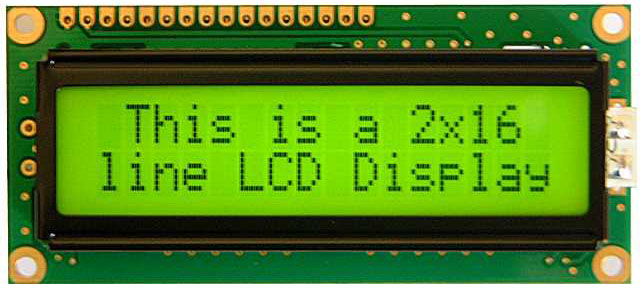
\includegraphics[height = 2cm]{figures/lcd.jpg}
\end{center} 

Nematic phase:
\begin{itemize}
\item No positional order
\item Orientational order
\end{itemize}
\vspace{-0.5cm}
\center 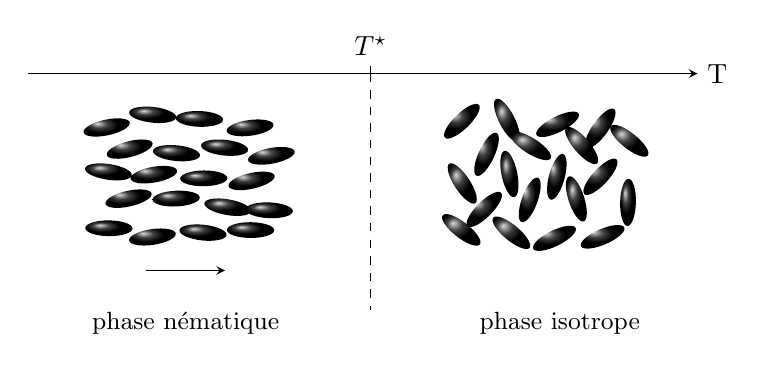
\begin{tikzpicture}[radius=0.1]
	\draw [->, >=stealth] (-1,2) -- (7.5,2) node[right]{T};
	\draw (3.35,1.9) -- (3.35,2.1) node[above]{$T^\star$};
	\draw [dashed] (3.35,2) -- (3.35,-1);

	\pgfmathsetseed{100}
	\pgfmathsetmacro{\xi}{0};
	\pgfmathsetmacro{\yi}{0};
	\foreach \i in {0,...,3}{
		\foreach \j in {0,...,2}{
			\pgfmathsetmacro{\x}{\xi+\i*0.6+0.04*rand};
			\pgfmathsetmacro{\y}{\yi+\j*0.7+0.1*rand};
			\pgfmathsetmacro{\angle}{rand*15};
			\drawZnema{\x}{\y}{\angle};
		}
	}
	\foreach \i in {0,...,3}{
		\foreach \j in {0,...,1}{
			\pgfmathsetmacro{\x}{\xi+0.3+\i*0.6+0.04*rand};
			\pgfmathsetmacro{\y}{\yi+0.35+\j*0.7+0.1*rand};
			\pgfmathsetmacro{\angle}{rand*15};
			\drawZnema{\x}{\y}{\angle};
		}
	}
	\draw [->,>=stealth] (0.5,-0.5) -- (1.5,-0.5);

	\pgfmathsetseed{79}
	\pgfmathsetmacro{\xi}{4.5};
	\pgfmathsetmacro{\yi}{0};
	\foreach \i in {0,...,3}{
		\foreach \j in {0,...,2}{
			\pgfmathsetmacro{\x}{\xi+\i*0.6+0.04*rand};
			\pgfmathsetmacro{\y}{\yi+\j*0.7+0.1*rand};
			\pgfmathsetmacro{\angle}{rand*180};
			\drawZnema{\x}{\y}{\angle};
		}
	}
	\foreach \i in {0,...,3}{
		\foreach \j in {0,...,1}{
			\pgfmathsetmacro{\x}{\xi+0.3+\i*0.6+0.04*rand};
			\pgfmathsetmacro{\y}{\yi+0.35+\j*0.7+0.1*rand};
			\pgfmathsetmacro{\angle}{rand*180};
			\drawZnema{\x}{\y}{\angle};
		}
	}


	\draw (1,-0.9) node[below]{\small phase nématique};
	\draw (5.75,-0.9) node[below]{\small phase isotrope};
\end{tikzpicture}


\end{frame}
%%%%%%%%%%%%%


%%%%%%%%%%%%% Slide de sommaire
\begin{frame}
	\frametitle{Sommaire}
	\framesubtitle{\ }
	\tableofcontents
\end{frame}
%%%%%%%%%%%%%

\section{The order parameter}

%%%%%%%%%%%%% 
\begin{frame}
	\frametitle{The Order Parameter}
	\framesubtitle{\ }
	
\center 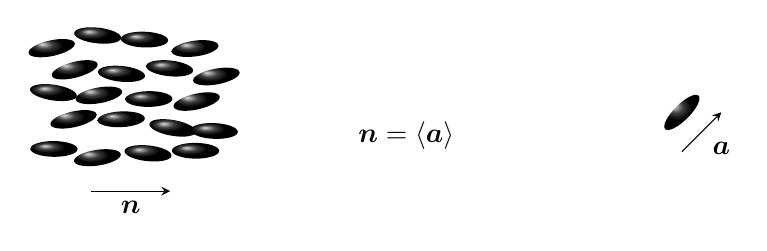
\begin{tikzpicture}[radius=0.1]


	\pgfmathsetseed{100}
	\pgfmathsetmacro{\xi}{-5};
	\pgfmathsetmacro{\yi}{0};
	\foreach \i in {0,...,3}{
		\foreach \j in {0,...,2}{
			\pgfmathsetmacro{\x}{\xi+\i*0.6+0.04*rand};
			\pgfmathsetmacro{\y}{\yi+\j*0.7+0.1*rand};
			\pgfmathsetmacro{\angle}{rand*15};
			\drawZnema{\x}{\y}{\angle};
		}
	}
	\foreach \i in {0,...,3}{
		\foreach \j in {0,...,1}{
			\pgfmathsetmacro{\x}{\xi+0.3+\i*0.6+0.04*rand};
			\pgfmathsetmacro{\y}{\yi+0.35+\j*0.7+0.1*rand};
			\pgfmathsetmacro{\angle}{rand*15};
			\drawZnema{\x}{\y}{\angle};
		}
	}

	\draw [->,>=stealth] (-4.5,-0.5) -- (-3.5,-0.5);
	\draw (-4,-0.5) node[below]{$\boldsymbol{n}$};

    \pgfmathsetmacro{\angle}{45};
    \drawZnema{3}{0.5}{\angle};
    \draw [->,>=stealth] (3,0) -- (3.5,0.5);
    \draw (3.5,0.25) node[below]{$\boldsymbol{a}$};

    \draw (-0.5,0.5) node[below]{ $\boldsymbol{n} = \langle \boldsymbol{a} \rangle $};

\end{tikzpicture}




\begin{equation*}
S = \frac{3 \langle (\bm{a}\cdot \bm{n})^2\rangle -1}{2}
\end{equation*}

\vspace{0.75cm}
Nematic phase : $S=1$ \hspace{0.9cm}
Isotropic phase : $S=0$
\end{frame}
%%%%%%%%%%%%%

\section{Numerical methods}
\subsection{Lebwohl Lasher Model}
%%%%%%%%%%%%% 
\begin{frame}
	\frametitle{Numerical Methods}
	\framesubtitle{Lebwohl Lasher Model}

\begin{textblock*}{13cm}(0cm,0.75cm) % {block width} (coords)
\begin{center}
	
\begin{tikzpicture}

    \pgfmathsetseed{1}
    

    \foreach \i in {0,...,5}{
        \pgfmathsetmacro{\x}{\i*0.7};
        \draw (\x,0) -- (\x,0.7*5);
        \draw (0,\x) -- (0.7*5,\x);
    }

    \foreach \i in {0,...,5}{
    \pgfmathsetmacro{\x}{\i*0.7};
        \foreach \j in {0,1,5}{
            
            \pgfmathsetmacro{\y}{\j*0.7};
            \pgfmathsetmacro{\angle}{rand*60};
            \pgfmathsetmacro{\size}{0.3};
            \drawNema{\x}{\y}{\angle}{\size};
        }
    }

    \foreach \j in {4,2,3}{
        \pgfmathsetmacro{\y}{\j*0.7};
        \foreach \i in {0,4,5}{
            \pgfmathsetmacro{\x}{\i*0.7};
            \pgfmathsetmacro{\angle}{rand*60};
            \pgfmathsetmacro{\size}{0.3};
            \drawNema{\x}{\y}{\angle}{\size};
        }
    }


    \pgfmathsetmacro{\xc}{2*0.7};
    \pgfmathsetmacro{\yc}{3*0.7};
    \pgfmathsetmacro{\anglec}{rand*60};
    \pgfmathsetmacro{\sizec}{0.3};

    \pgfmathsetmacro{\xul}{1*0.7};
    \pgfmathsetmacro{\yul}{4*0.7};
    \pgfmathsetmacro{\angleul}{rand*60};
    \pgfmathsetmacro{\sizeul}{0.3};

    \pgfmathsetmacro{\xum}{2*0.7};
    \pgfmathsetmacro{\yum}{4*0.7};
    \pgfmathsetmacro{\angleum}{rand*60};
    \pgfmathsetmacro{\sizeum}{0.3};

    \pgfmathsetmacro{\xur}{3*0.7};
    \pgfmathsetmacro{\yur}{4*0.7};
    \pgfmathsetmacro{\angleur}{rand*60};
    \pgfmathsetmacro{\sizeur}{0.3};

    \pgfmathsetmacro{\xmr}{1*0.7};
    \pgfmathsetmacro{\ymr}{3*0.7};
    \pgfmathsetmacro{\anglemr}{rand*60};
    \pgfmathsetmacro{\sizemr}{0.3};

    \pgfmathsetmacro{\xml}{3*0.7};
    \pgfmathsetmacro{\yml}{3*0.7};
    \pgfmathsetmacro{\angleml}{rand*60};
    \pgfmathsetmacro{\sizeml}{0.3};

    \pgfmathsetmacro{\xdl}{1*0.7};
    \pgfmathsetmacro{\ydl}{2*0.7};
    \pgfmathsetmacro{\angledl}{rand*60};
    \pgfmathsetmacro{\sizedl}{0.3};

    \pgfmathsetmacro{\xdr}{3*0.7};
    \pgfmathsetmacro{\ydr}{2*0.7};
    \pgfmathsetmacro{\angledr}{rand*60};
    \pgfmathsetmacro{\sizedr}{0.3};

    \pgfmathsetmacro{\xdm}{2*0.7};
    \pgfmathsetmacro{\ydm}{2*0.7};
    \pgfmathsetmacro{\angledm}{rand*60};
    \pgfmathsetmacro{\sizedm}{0.3};

            \drawNema{\xul}{\yul}{\angleul}{\sizeul};
            \drawNema{\xum}{\yum}{\angleum}{\sizeum};
            \drawNema{\xur}{\yur}{\angleur}{\sizeur};

            \drawNema{\xml}{\yml}{\angleml}{\sizeml};
            \drawNema{\xmr}{\ymr}{\anglemr}{\sizemr};

            \drawNema{\xdr}{\ydr}{\angledr}{\sizedr};
            \drawNema{\xdl}{\ydl}{\angledl}{\sizedl};
            \drawNema{\xdm}{\ydm}{\angledm}{\sizedm};

            \drawNema{\xc}{\yc}{\anglec}{\sizec};
    


\end{tikzpicture}

\end{center}
\end{textblock*}

\begin{textblock*}{13cm}(0cm,5cm) % {block width} (coords)
\begin{center}
	Size : $ 30 \times 30 \times 30$
\end{center}
\end{textblock*}

\begin{textblock*}{13cm}(0cm,7cm) % {block width} (coords)
\begin{equation*}
E = - \epsilon\sum_{<i,j>} \frac{3\cos^2\alpha_{i,j}-1}{2}
\end{equation*}
\end{textblock*}
\end{frame}
%%%%%%%%%%%%%

\subsection{Monte-Carlo Algorithm}
%%%%%%%%%%%%% 
\begin{frame}
	\frametitle{Numerical Methods}
	\framesubtitle{Monte-Carlo Algorithm}

\begin{textblock*}{13cm}(0cm,0.75cm) % {block width} (coords)
\begin{center}
	
\begin{tikzpicture}

\pgfmathsetseed{1}
    
    \onslide<1-7> {
    \foreach \i in {0,...,5}{
        \pgfmathsetmacro{\x}{\i*0.7};
        \draw (\x,0) -- (\x,0.7*5);
        \draw (0,\x) -- (0.7*5,\x);
    }

	\foreach \i in {0,...,5}{
    \pgfmathsetmacro{\x}{\i*0.7};
		\foreach \j in {0,1,5}{
			
			\pgfmathsetmacro{\y}{\j*0.7};
			\pgfmathsetmacro{\angle}{rand*60};
            \pgfmathsetmacro{\size}{0.3};
			\drawNema{\x}{\y}{\angle}{\size};
		}
	}

    \foreach \j in {4,2,3}{
        \pgfmathsetmacro{\y}{\j*0.7};
        \foreach \i in {0,4,5}{
            \pgfmathsetmacro{\x}{\i*0.7};
            \pgfmathsetmacro{\angle}{rand*60};
            \pgfmathsetmacro{\size}{0.3};
            \drawNema{\x}{\y}{\angle}{\size};
        }
    }
    }

    \pgfmathsetmacro{\xc}{2*0.7};
    \pgfmathsetmacro{\yc}{3*0.7};
    \pgfmathsetmacro{\anglec}{rand*60};
    \pgfmathsetmacro{\sizec}{0.3};

    \pgfmathsetmacro{\xul}{1*0.7};
    \pgfmathsetmacro{\yul}{4*0.7};
    \pgfmathsetmacro{\angleul}{rand*60};
    \pgfmathsetmacro{\sizeul}{0.3};

    \pgfmathsetmacro{\xum}{2*0.7};
    \pgfmathsetmacro{\yum}{4*0.7};
    \pgfmathsetmacro{\angleum}{rand*60};
    \pgfmathsetmacro{\sizeum}{0.3};

    \pgfmathsetmacro{\xur}{3*0.7};
    \pgfmathsetmacro{\yur}{4*0.7};
    \pgfmathsetmacro{\angleur}{rand*60};
    \pgfmathsetmacro{\sizeur}{0.3};

    \pgfmathsetmacro{\xmr}{1*0.7};
    \pgfmathsetmacro{\ymr}{3*0.7};
    \pgfmathsetmacro{\anglemr}{rand*60};
    \pgfmathsetmacro{\sizemr}{0.3};

    \pgfmathsetmacro{\xml}{3*0.7};
    \pgfmathsetmacro{\yml}{3*0.7};
    \pgfmathsetmacro{\angleml}{rand*60};
    \pgfmathsetmacro{\sizeml}{0.3};

    \pgfmathsetmacro{\xdl}{1*0.7};
    \pgfmathsetmacro{\ydl}{2*0.7};
    \pgfmathsetmacro{\angledl}{rand*60};
    \pgfmathsetmacro{\sizedl}{0.3};

    \pgfmathsetmacro{\xdr}{3*0.7};
    \pgfmathsetmacro{\ydr}{2*0.7};
    \pgfmathsetmacro{\angledr}{rand*60};
    \pgfmathsetmacro{\sizedr}{0.3};

    \pgfmathsetmacro{\xdm}{2*0.7};
    \pgfmathsetmacro{\ydm}{2*0.7};
    \pgfmathsetmacro{\angledm}{rand*60};
    \pgfmathsetmacro{\sizedm}{0.3};

    \onslide<1-2,7> {
            \drawNema{\xul}{\yul}{\angleul}{\sizeul};
            \drawNema{\xum}{\yum}{\angleum}{\sizeum};
            \drawNema{\xur}{\yur}{\angleur}{\sizeur};

            \drawNema{\xml}{\yml}{\angleml}{\sizeml};
            \drawNema{\xmr}{\ymr}{\anglemr}{\sizemr};

            \drawNema{\xdr}{\ydr}{\angledr}{\sizedr};
            \drawNema{\xdl}{\ydl}{\angledl}{\sizedl};
            \drawNema{\xdm}{\ydm}{\angledm}{\sizedm};
    }

    \onslide<1> {
        \drawNema{\xc}{\yc}{\anglec}{\sizec};
    }

    \onslide<2-4> {
        \drawblueNema{\xc}{\yc}{\anglec}{\sizec};
    }

    \onslide<3> {
            \drawgreenNema{\xul}{\yul}{\angleul}{\sizeul};
            \drawgreenNema{\xum}{\yum}{\angleum}{\sizeum};
            \drawgreenNema{\xur}{\yur}{\angleur}{\sizeur};

            \drawgreenNema{\xml}{\yml}{\angleml}{\sizeml};
            \drawgreenNema{\xmr}{\ymr}{\anglemr}{\sizemr};

            \drawgreenNema{\xdr}{\ydr}{\angledr}{\sizedr};
            \drawgreenNema{\xdl}{\ydl}{\angledl}{\sizedl};
            \drawgreenNema{\xdm}{\ydm}{\angledm}{\sizedm};
    }

    \onslide<4-5> {
            \drawNema{\xul}{\yul}{\angleul}{\sizeul};
            \drawNema{\xum}{\yum}{\angleum}{\sizeum};
            \drawNema{\xur}{\yur}{\angleur}{\sizeur};

            \drawNema{\xml}{\yml}{\angleml}{\sizeml};
            \drawNema{\xmr}{\ymr}{\anglemr}{\sizemr};

            \drawNema{\xdr}{\ydr}{\angledr}{\sizedr};
            \drawNema{\xdl}{\ydl}{\angledl}{\sizedl};
            \drawNema{\xdm}{\ydm}{\angledm}{\sizedm};
    }

    \pgfmathsetmacro{\anglec}{\anglec +90};
    \onslide<5-7> {
        \drawredNema{\xc}{\yc}{\anglec}{\sizec};
    }

    \onslide<6> {
            \drawgreenNema{\xul}{\yul}{\angleul}{\sizeul};
            \drawgreenNema{\xum}{\yum}{\angleum}{\sizeum};
            \drawgreenNema{\xur}{\yur}{\angleur}{\sizeur};

            \drawgreenNema{\xml}{\yml}{\angleml}{\sizeml};
            \drawgreenNema{\xmr}{\ymr}{\anglemr}{\sizemr};

            \drawgreenNema{\xdr}{\ydr}{\angledr}{\sizedr};
            \drawgreenNema{\xdl}{\ydl}{\angledl}{\sizedl};
            \drawgreenNema{\xdm}{\ydm}{\angledm}{\sizedm};
    }

\end{tikzpicture}

\end{center}
\end{textblock*}

\only<2>{
\begin{textblock*}{10cm}(1.5cm,5cm) % {block width} (coords)
\begin{itemize}
\item We select a random site
\end{itemize}
\end{textblock*}
}

\only<3>{
\begin{textblock*}{10cm}(1.5cm,5cm) % {block width} (coords)
\begin{itemize}
\item We select a random site
\item We compute the energy with the neighboor : $\textcolor{blue}{E_{old}}$
\end{itemize}
\end{textblock*}
}


\only<4-5>{
\begin{textblock*}{10cm}(1.5cm,5cm) % {block width} (coords)
\begin{itemize}
\item We select a random site
\item We compute the energy with the neighboor : $\textcolor{blue}{E_{old}}$
\item We try to swap the chosen site
\end{itemize}
\end{textblock*}
}

\only<6>{
\begin{textblock*}{10cm}(1.5cm,5cm) % {block width} (coords)
\begin{itemize}
\item We select a random site
\item We compute the energy with the neighboor : $\textcolor{blue}{E_{old}}$
\item We try to swap the chosen site
\item We compute the energy with the neighboor : $\textcolor{red}{E_{new}}$
\end{itemize}
\end{textblock*}
}

\only<7>{
\begin{textblock*}{10cm}(1.5cm,5cm) % {block width} (coords)
\begin{itemize}
\item We select a random site
\item We compute the energy with the neighboor : $\textcolor{blue}{E_{old}}$
\item We try to swap the chosen site
\item We compute the energy with the neighboor : $\textcolor{red}{E_{new}}$
\item We accept the swap with a probability :
\vspace{-0.3cm}
\begin{equation*}
p = e^{-\dfrac{\textcolor{blue}{E_{old}} -\textcolor{red}{E_{new}}}{k_B T}}
\end{equation*}



\end{itemize}
\end{textblock*}
}

\end{frame}
%%%%%%%%%%%%%

\subsection{Equilibration}
%%%%%%%%%%%%% 
\begin{frame}
	\frametitle{Numerical Methods}
	\framesubtitle{Equilibration}

\begin{figure}
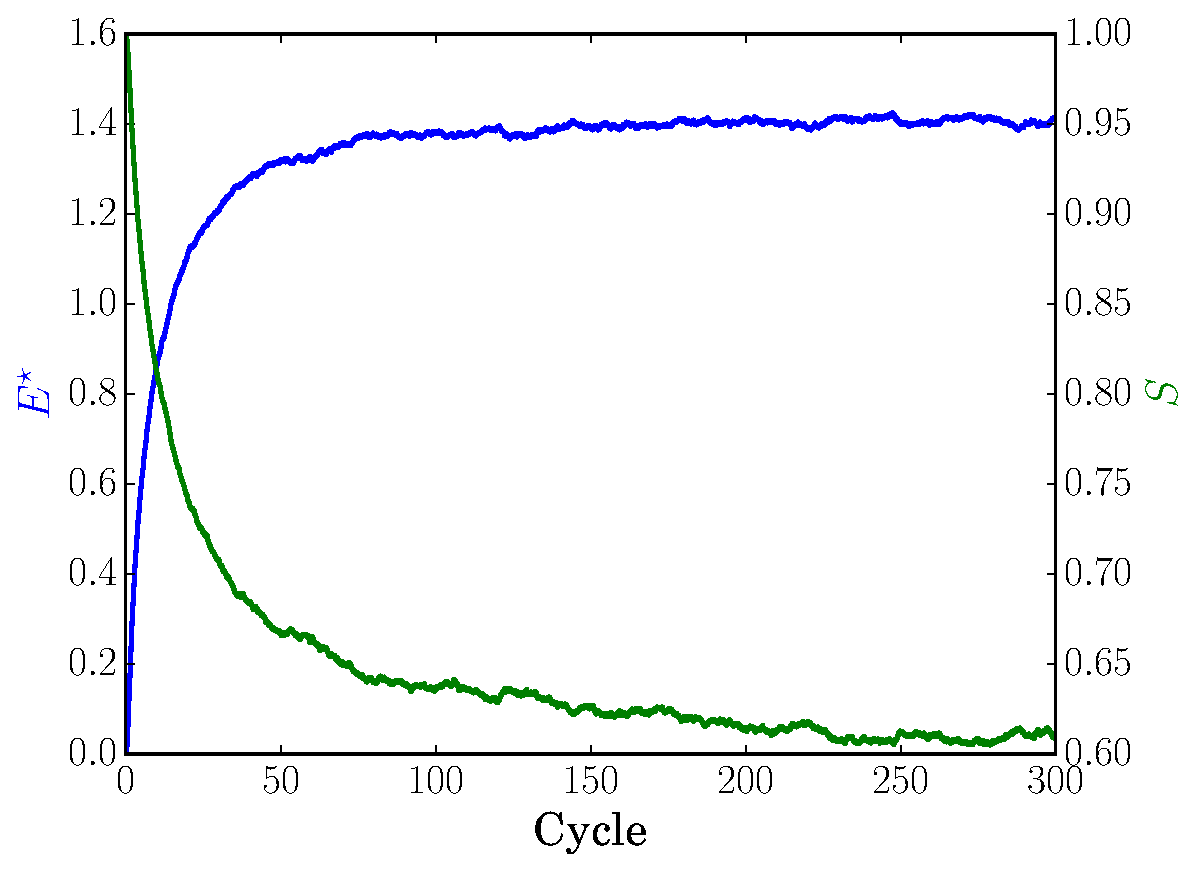
\includegraphics[scale=0.48]{figures/equilibrage.pdf}
\end{figure}
\vspace{-0.6cm}
\center Equilibration at $T^\star = 1$
\end{frame}
%%%%%%%%%%%%%

\section{Nematic Isotropic Phase Transitions}
\subsection{Direct visualisation}
%%%%%%%%%%%%% 
\begin{frame}
	\frametitle{Nematic Isotropic Phase Transitions}
	\framesubtitle{Direct visualisation}

\begin{columns}
    \begin{column}{3cm}
    	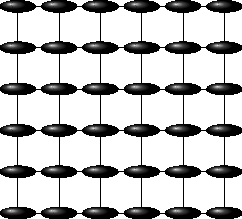
\includegraphics[scale=0.8]{figures/00.pdf}
	\end{column}

	\begin{column}{3cm}
    	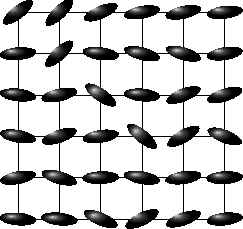
\includegraphics[scale=0.8]{figures/09.pdf}
	\end{column}
	
	\begin{column}{3cm}
    	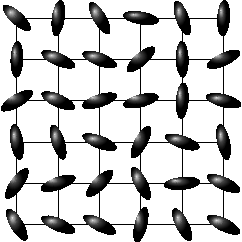
\includegraphics[scale=0.8]{figures/15.pdf}
	\end{column}
\end{columns}

\begin{columns}
    \begin{column}{3cm}
    	\center $T^\star =  0.05$
	\end{column}

	\begin{column}{3cm}
    	\center $T^\star =  0.9$
	\end{column}
	
	\begin{column}{3cm}
    	\center $T^\star =  1.5$
	\end{column}
\end{columns}

\end{frame}
%%%%%%%%%%%%%

\subsection{Energy}
%%%%%%%%%%%%% 
\begin{frame}
	\frametitle{Nematic Isotropic Phase Transitions}
	\framesubtitle{Energy}

\begin{figure}
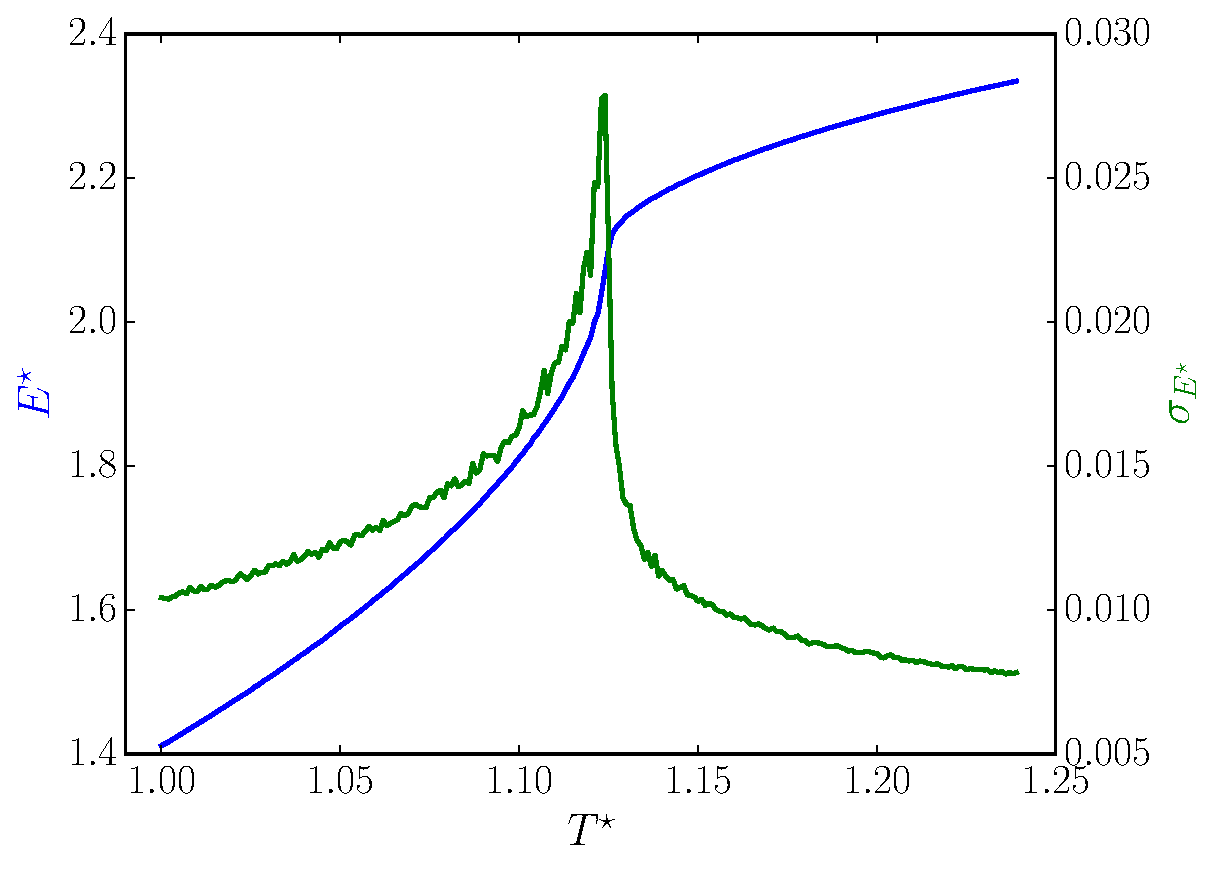
\includegraphics[scale=0.48]{figures/local_energie.pdf}
\end{figure}
\vspace{-0.6cm}
\center Energy and its variance.
\end{frame}
%%%%%%%%%%%%%

\subsection{Energy}
%%%%%%%%%%%%% 
\begin{frame}
	\frametitle{Nematic Isotropic Phase Transitions}
	\framesubtitle{Energy}

\begin{figure}
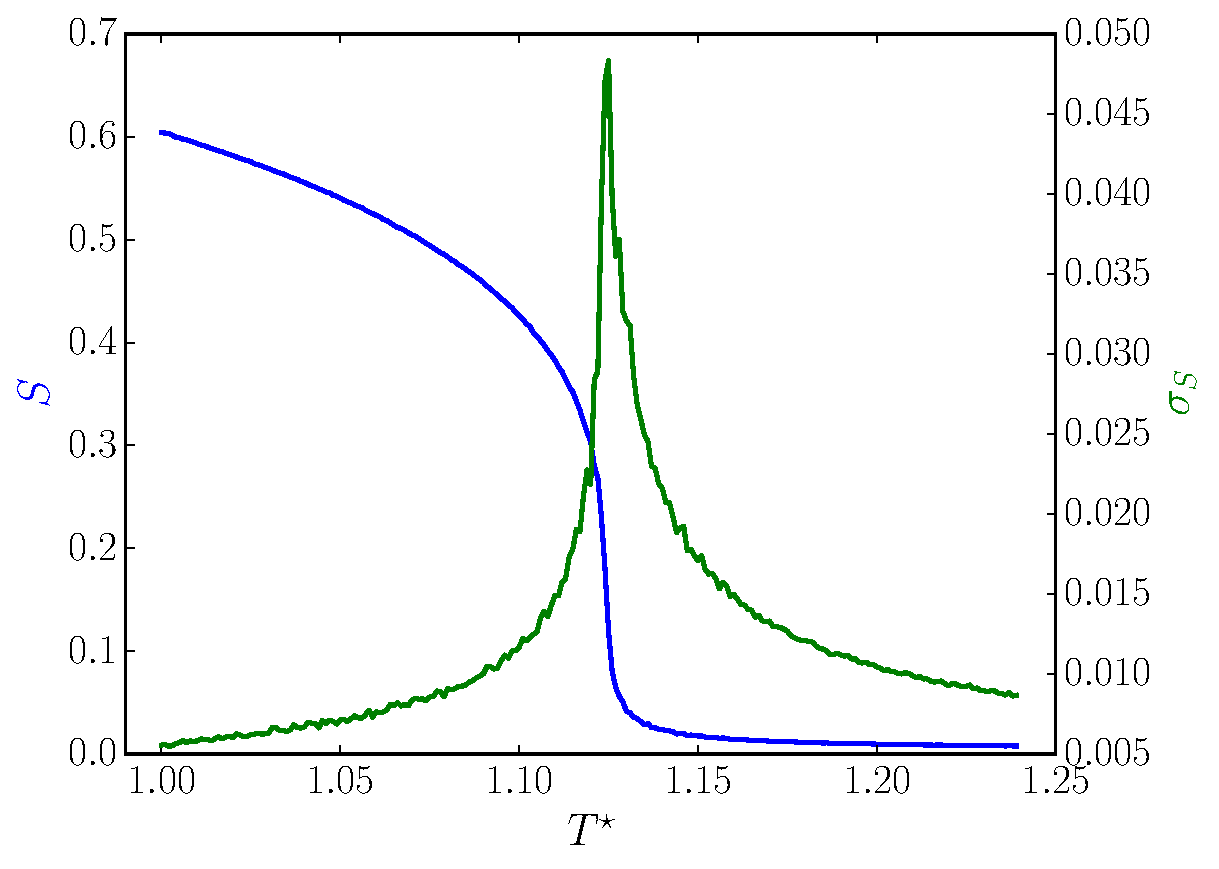
\includegraphics[scale=0.48]{figures/local_order.pdf}
\end{figure}
\vspace{-0.6cm}
\center Order parameter and its variance.
\end{frame}
%%%%%%%%%%%%%

\subsection{Histograms}
%%%%%%%%%%%%% 
\begin{frame}
	\frametitle{Nematic Isotropic Phase Transitions}
	\framesubtitle{Energy Histograms}
\vspace{-0.3cm}
\begin{columns}
    \begin{column}{6cm}
    \center
    	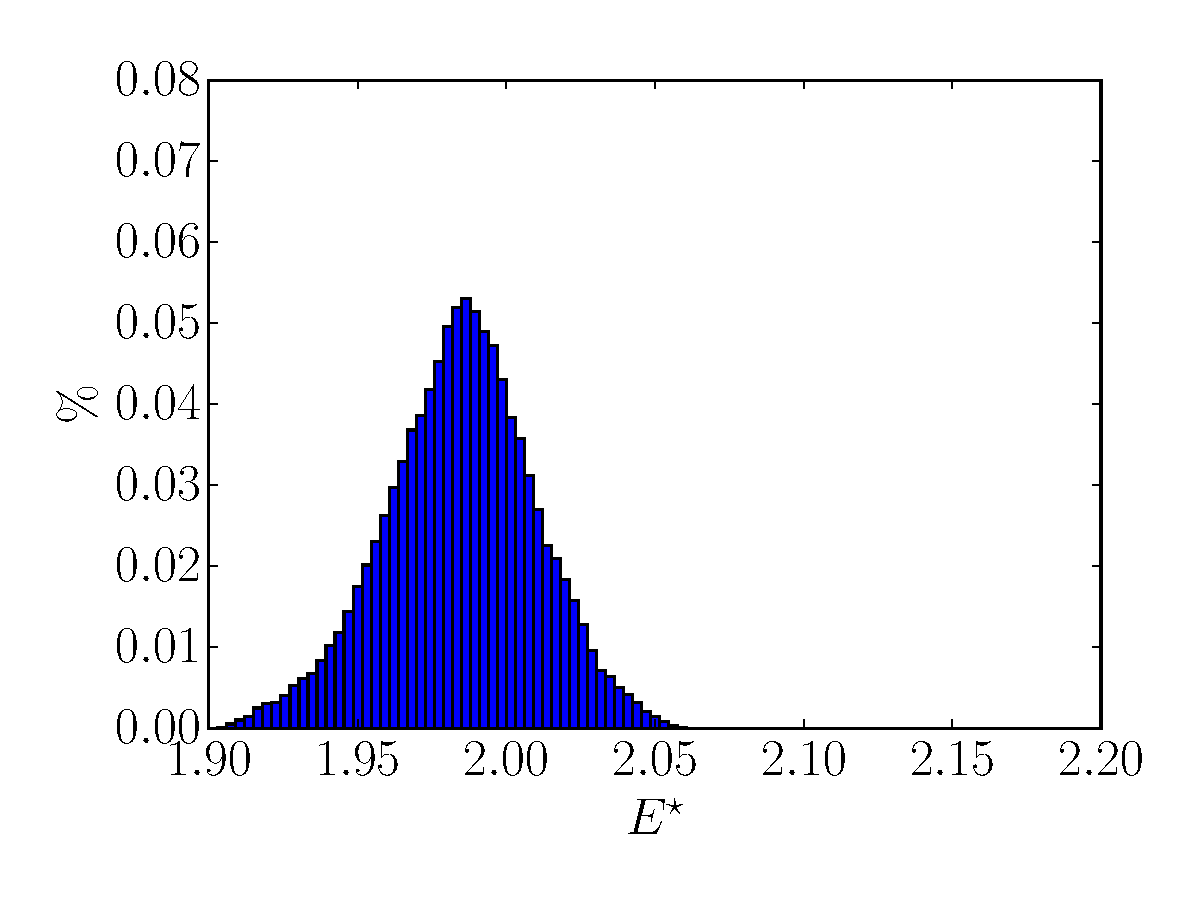
\includegraphics[scale=0.28]{figures/histo_11208.pdf}
	\end{column}

	\begin{column}{6cm}
	\center
    	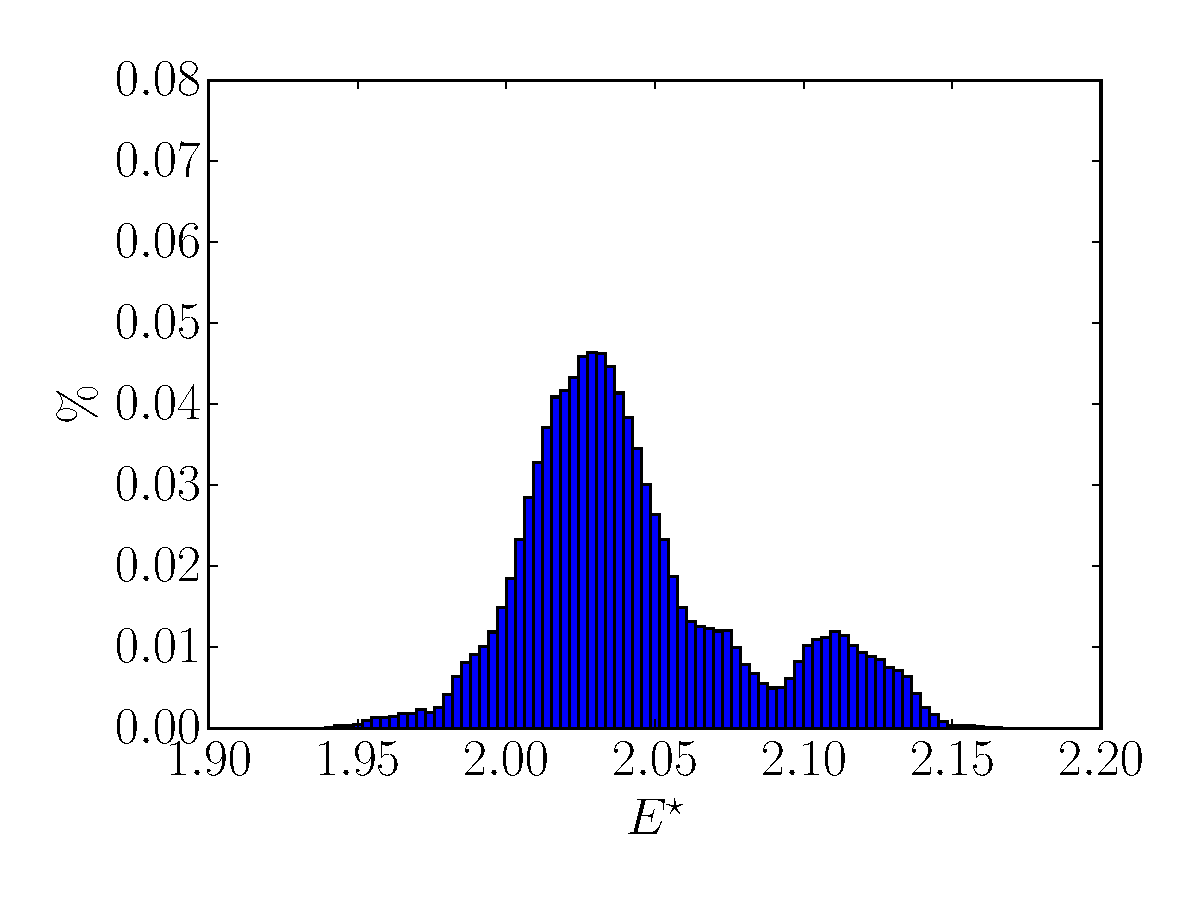
\includegraphics[scale=0.28]{figures/histo_11228.pdf}
	\end{column}

\end{columns}
\vspace{-0.7cm}

\begin{columns}
    \begin{column}{6cm}
    \center
    	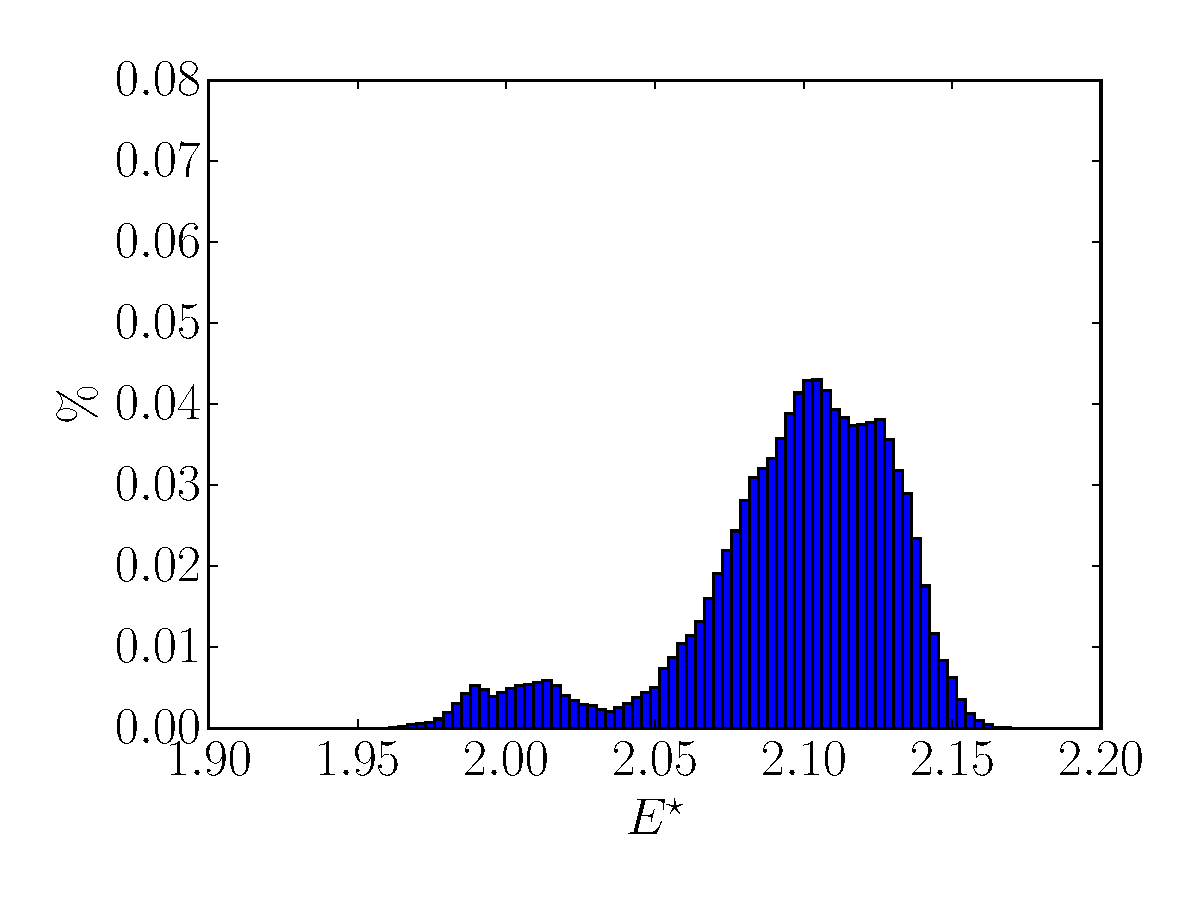
\includegraphics[scale=0.28]{figures/histo_11240.pdf}
	\end{column}

	\begin{column}{6cm}
	\center
    	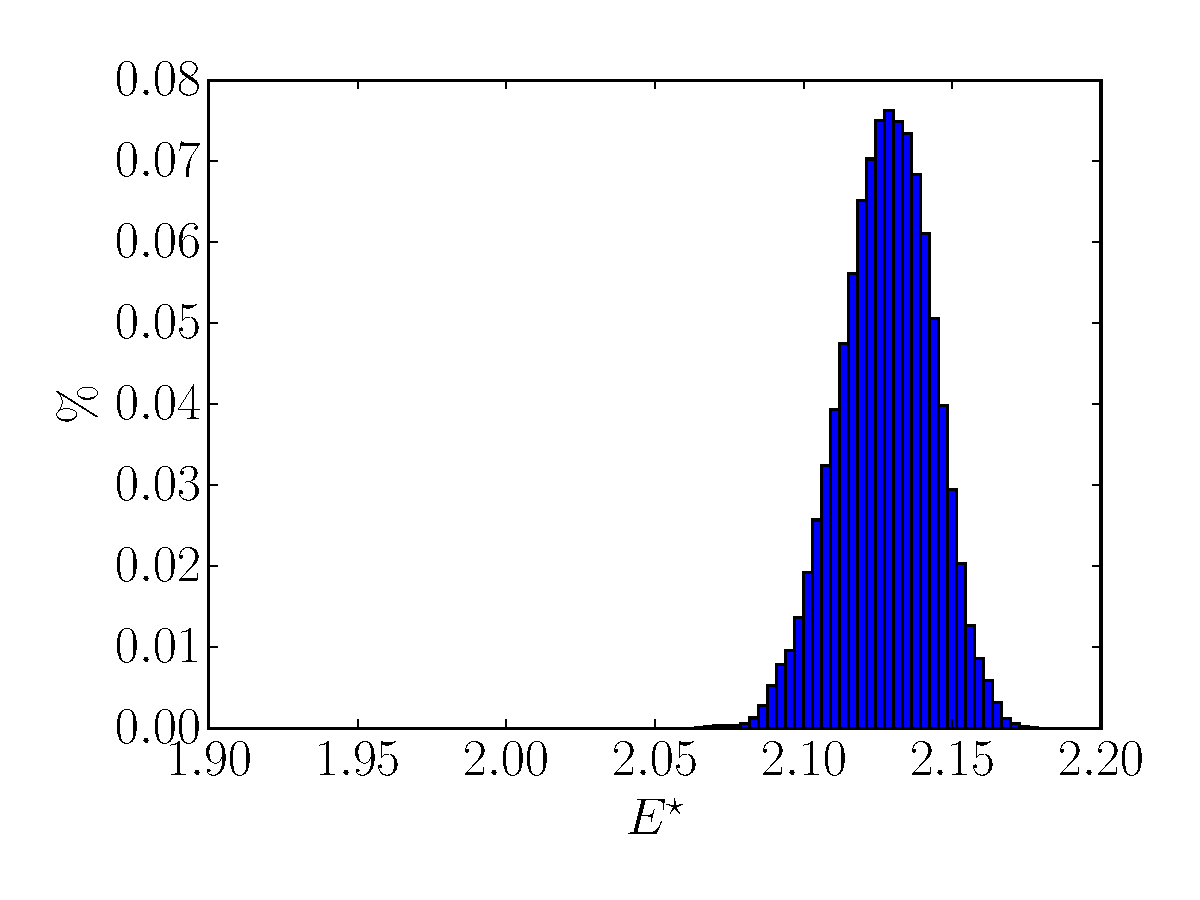
\includegraphics[scale=0.28]{figures/histo_11256.pdf}
	\end{column}

\end{columns}

\end{frame}
%%%%%%%%%%%%%


\section{Influence of an Electric Field}
\subsection{Lebwohl Lasher Model}
%%%%%%%%%%%%% 
\begin{frame}
	\frametitle{Numerical Methods}
	\framesubtitle{Lebwohl Lasher Model}

\begin{textblock*}{13cm}(0cm,0.75cm) % {block width} (coords)
\begin{center}
	
\begin{tikzpicture}

    \pgfmathsetseed{1}
    

    \foreach \i in {0,...,5}{
        \pgfmathsetmacro{\x}{\i*0.7};
        \draw (\x,0) -- (\x,0.7*5);
        \draw (0,\x) -- (0.7*5,\x);
    }

    \foreach \i in {0,...,5}{
    \pgfmathsetmacro{\x}{\i*0.7};
        \foreach \j in {0,1,5}{
            
            \pgfmathsetmacro{\y}{\j*0.7};
            \pgfmathsetmacro{\angle}{rand*60};
            \pgfmathsetmacro{\size}{0.3};
            \drawNema{\x}{\y}{\angle}{\size};
        }
    }

    \foreach \j in {4,2,3}{
        \pgfmathsetmacro{\y}{\j*0.7};
        \foreach \i in {0,4,5}{
            \pgfmathsetmacro{\x}{\i*0.7};
            \pgfmathsetmacro{\angle}{rand*60};
            \pgfmathsetmacro{\size}{0.3};
            \drawNema{\x}{\y}{\angle}{\size};
        }
    }


    \pgfmathsetmacro{\xc}{2*0.7};
    \pgfmathsetmacro{\yc}{3*0.7};
    \pgfmathsetmacro{\anglec}{rand*60};
    \pgfmathsetmacro{\sizec}{0.3};

    \pgfmathsetmacro{\xul}{1*0.7};
    \pgfmathsetmacro{\yul}{4*0.7};
    \pgfmathsetmacro{\angleul}{rand*60};
    \pgfmathsetmacro{\sizeul}{0.3};

    \pgfmathsetmacro{\xum}{2*0.7};
    \pgfmathsetmacro{\yum}{4*0.7};
    \pgfmathsetmacro{\angleum}{rand*60};
    \pgfmathsetmacro{\sizeum}{0.3};

    \pgfmathsetmacro{\xur}{3*0.7};
    \pgfmathsetmacro{\yur}{4*0.7};
    \pgfmathsetmacro{\angleur}{rand*60};
    \pgfmathsetmacro{\sizeur}{0.3};

    \pgfmathsetmacro{\xmr}{1*0.7};
    \pgfmathsetmacro{\ymr}{3*0.7};
    \pgfmathsetmacro{\anglemr}{rand*60};
    \pgfmathsetmacro{\sizemr}{0.3};

    \pgfmathsetmacro{\xml}{3*0.7};
    \pgfmathsetmacro{\yml}{3*0.7};
    \pgfmathsetmacro{\angleml}{rand*60};
    \pgfmathsetmacro{\sizeml}{0.3};

    \pgfmathsetmacro{\xdl}{1*0.7};
    \pgfmathsetmacro{\ydl}{2*0.7};
    \pgfmathsetmacro{\angledl}{rand*60};
    \pgfmathsetmacro{\sizedl}{0.3};

    \pgfmathsetmacro{\xdr}{3*0.7};
    \pgfmathsetmacro{\ydr}{2*0.7};
    \pgfmathsetmacro{\angledr}{rand*60};
    \pgfmathsetmacro{\sizedr}{0.3};

    \pgfmathsetmacro{\xdm}{2*0.7};
    \pgfmathsetmacro{\ydm}{2*0.7};
    \pgfmathsetmacro{\angledm}{rand*60};
    \pgfmathsetmacro{\sizedm}{0.3};

            \drawNema{\xul}{\yul}{\angleul}{\sizeul};
            \drawNema{\xum}{\yum}{\angleum}{\sizeum};
            \drawNema{\xur}{\yur}{\angleur}{\sizeur};

            \drawNema{\xml}{\yml}{\angleml}{\sizeml};
            \drawNema{\xmr}{\ymr}{\anglemr}{\sizemr};

            \drawNema{\xdr}{\ydr}{\angledr}{\sizedr};
            \drawNema{\xdl}{\ydl}{\angledl}{\sizedl};
            \drawNema{\xdm}{\ydm}{\angledm}{\sizedm};

            \drawNema{\xc}{\yc}{\anglec}{\sizec};
    


\end{tikzpicture}

\end{center}
\end{textblock*}

\begin{textblock*}{13cm}(0cm,5cm) % {block width} (coords)
\center
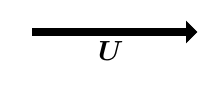
\begin{tikzpicture}[radius=0.1]
\path[draw=black,solid,line width=1.1mm,fill=black,
preaction={-triangle 90,thin,draw,shorten >=-1mm}
] (-1, 0) -- (1, 0);

\draw (0,0) node[below]{$\boldsymbol{U}$};
\end{tikzpicture}
\end{textblock*}

\begin{textblock*}{13cm}(0cm,7cm) % {block width} (coords)
\begin{equation*}
E = - \epsilon\sum_{<i,j>} \frac{3\cos^2\alpha_{i,j}-1}{2} - \epsilon \xi U^2 \sum_{i}\frac{3\cos^2\beta_i-1}{2}
\end{equation*}

\end{textblock*}
\end{frame}
%%%%%%%%%%%%%

\subsection{Critical point}
%%%%%%%%%%%%% 
\begin{frame}
	\frametitle{Numerical Methods}
	\framesubtitle{Energy}

\begin{figure}
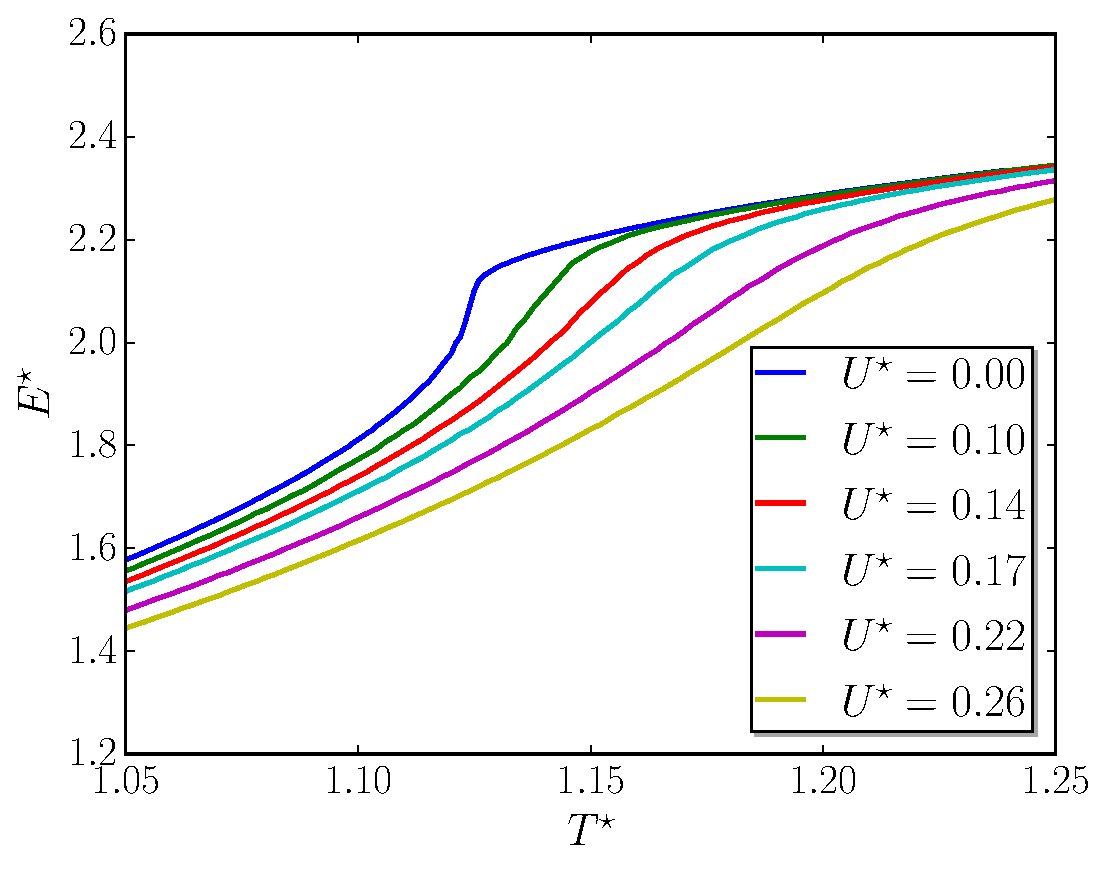
\includegraphics[scale=0.48]{figures/electricField_calo.pdf}
\end{figure}
\vspace{-0.6cm}
\center Energy for different electric field.
\end{frame}
%%%%%%%%%%%%%

\subsection{Phase diagram}
%%%%%%%%%%%%% 
\begin{frame}
	\frametitle{Numerical Methods}
	\framesubtitle{Phase diagram}

\begin{figure}
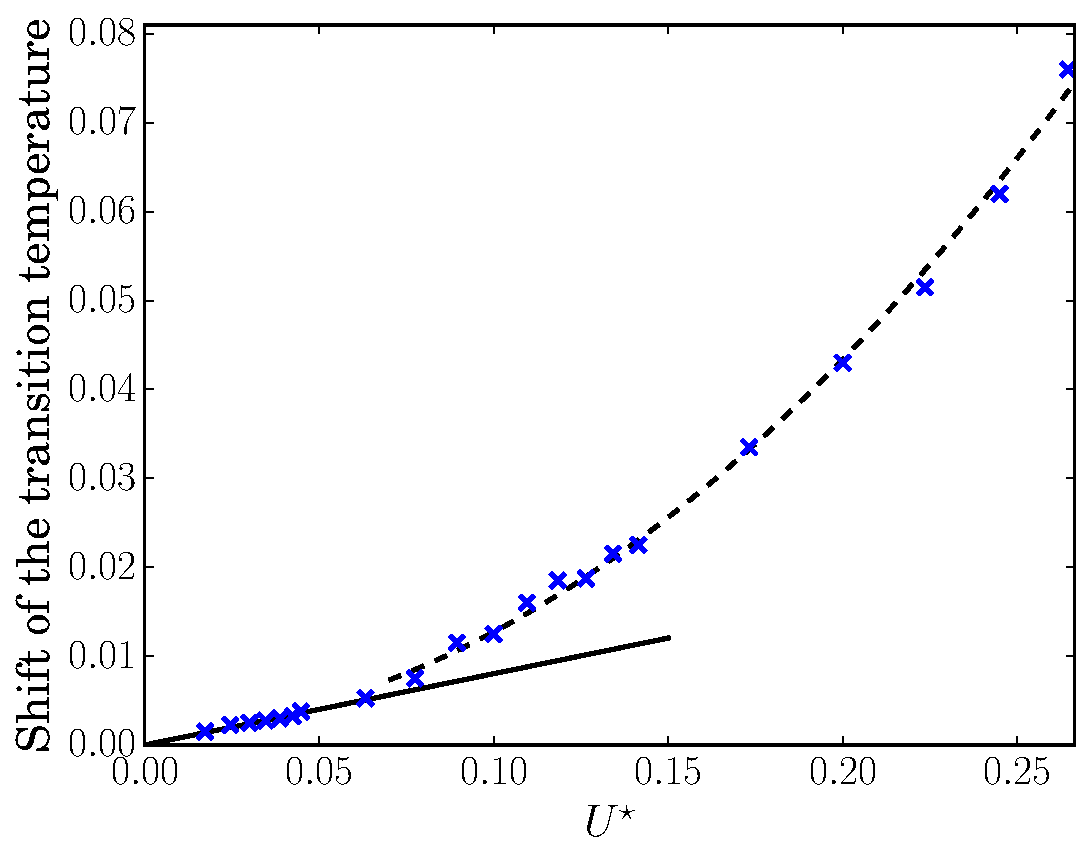
\includegraphics[scale=0.48]{figures/electricField.pdf}
\end{figure}
\vspace{-0.6cm}
\center Transition temperature as a function of the electric field.
\end{frame}
%%%%%%%%%%%%%


%%%%%%%%%%%%% 
\begin{frame}
	\frametitle{Conclusion}
	\framesubtitle{\ }
	

\end{frame}
%%%%%%%%%%%%%

%%%%%%%%%%%%% 
\begin{frame}
	\frametitle{Perspectives}
	\framesubtitle{\ }

\end{frame}
%%%%%%%%%%%%%



%%%%%%%%%%%%% 
\begin{frame}
	\frametitle{\ }
	\framesubtitle{\ }

{\center $\qquad$ \Huge Merci pour votre attention}

\end{frame}
%%%%%%%%%%%%%






%%%%%%%%%%%%%
\end{document}